% The flow chart created here depicts PyVVO's load modeling procedures.
\documentclass[tikz]{standalone}

\usepackage{amsmath}

% Load up the basic commands.
\usetikzlibrary{shapes.geometric, arrows.meta, fit, calc, positioning, automata, decorations.pathreplacing}

% When we exceed 26 characters...
% https://tex.stackexchange.com/a/269559/208656
\usepackage{alphalph}

% Declare the layers
% https://tex.stackexchange.com/a/75498/208656
\pgfdeclarelayer{background}
\pgfsetlayers{background,main}

% tikzset for flowcharts.
% https://tex.stackexchange.com/a/342227/208656
% Reference for label shifting in style:
% https://tex.stackexchange.com/a/78690/208656
% Reference for curly braces:
% https://tex.stackexchange.com/a/20887/208656
\tikzset{flowchart/.style = {
	base/.style = {
		draw=black,
		very thick,
		inner sep=10pt,
		outer sep=0pt,
		text width=10.0cm,
		minimum height=0.8cm,
		align=flush center,
	},
	labelshift/.style = {
		prefix after command= {\pgfextra{\tikzset{every label/.style={xshift=0.42cm}}}}
	},
	startstop/.style = {
		base,
		labelshift,
		rectangle,
		rounded corners,
		fill=red!30
	},
	io/.style = {
		base,
		trapezium,
		trapezium left angle=70,
		trapezium right angle=110,
		trapezium stretches=true,
		fill=blue!30,
	},
	process/.style = {
		base,
		labelshift,
		rectangle,
		fill=orange!30
	},
	decision/.style = {
		base,
		text width=3.0cm,
		diamond,
		aspect=1.2,
		fill=green!30
	},
	arrows.meta/.style = {
		very thick,
	 	-{Stealth[]}
	},
	curlybrace/.style = {%
		draw=black,
		decorate,
		very thick,
		decoration={brace, amplitude=20pt, raise=6pt, mirror},
	},
	curlynode/.style = {
		draw=none,
		black,
		midway,
		xshift=2.75cm,
		text width=3cm	
	},
	backgroundbox/.style = {
		draw=none,
		inner sep=0.8cm,
		ultra thick,
		dashed,
		fill opacity=0.4
	}
}}

% Shortcut for inline code:
% https://stackoverflow.com/a/21344989
\newcommand{\code}[1]{\texttt{#1}}

% Label counter for the flow chart.
\newcounter{ac}
\renewcommand{\theac}{\alphalph{\value{ac}}}
\newcommand{\ac}[1]{(\refstepcounter{ac}\alphalph{\value{ac}})\label{#1}}

% To put parentheses around references:
\newcommand{\acref}[1]{(\ref{#1})}

% The following are for extracing coordinates.
% https://tex.stackexchange.com/a/33706/208656
\newdimen\XCoord
\newdimen\YCoord
\newcommand*{\ExtractCoordinate}[1]{\path (#1); \pgfgetlastxy{\XCoord}{\YCoord};}%
\newcommand*{\ExtractCoordinateTwo}[1]{\path (#1); \pgfgetlastxy{\XCoordTwo}{\YCoordTwo};}%

% Dimension and command for labeling boxes.
\newdimen\XLabel
\newcommand{\LabelNode}[1]{\ExtractCoordinate{$(#1.east)$}; \node (#1-label) at (\XLabel, \YCoord) {\ac{flow:#1}};}

\begin{document}
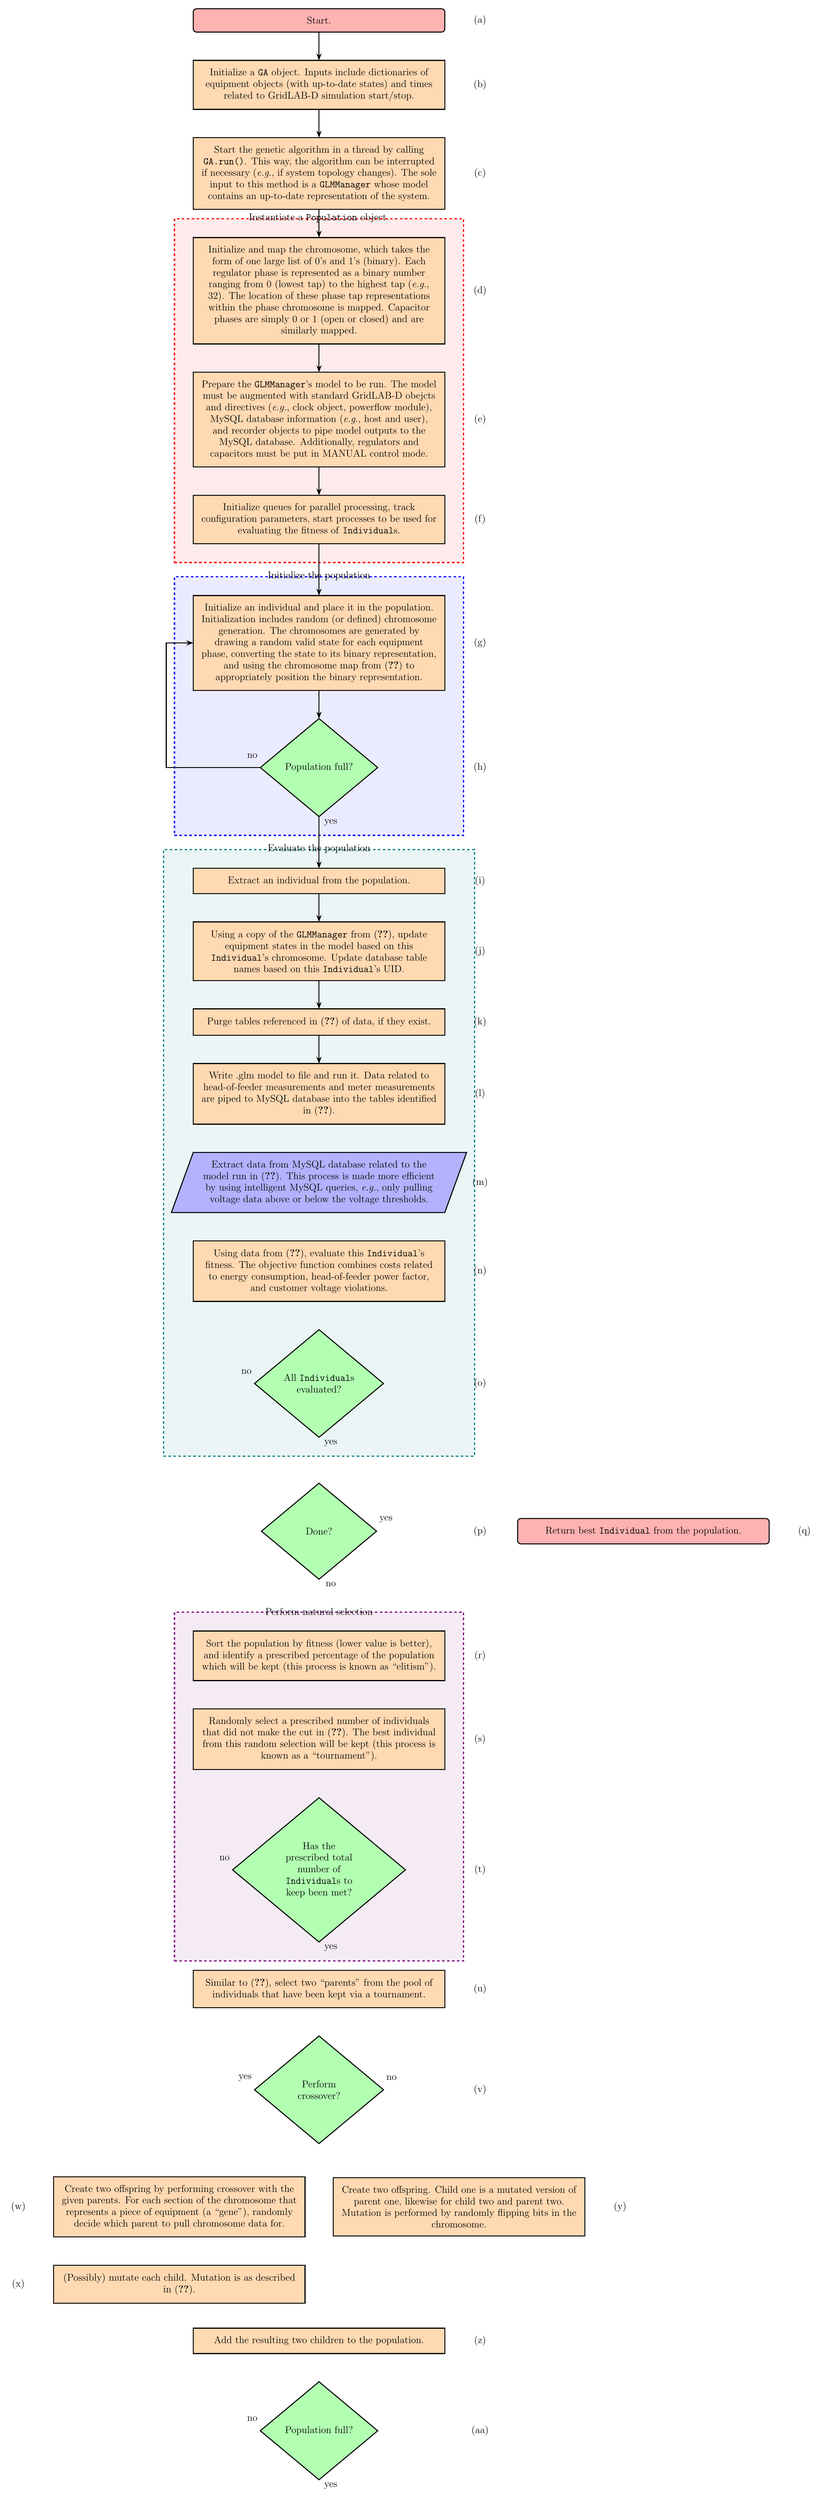
\begin{tikzpicture}[flowchart, node distance=1.2cm] 
\tikzstyle{every node}=[font=\large]

	%%%%%%%%%%%%%%%%%%%%%%%%%%%%%%%%%%%%%%%%%%%%%%%%%%%%%%%%%%%%%%%%
	% NODES AND ARROWS
	%%%%%%%%%%%%%%%%%%%%%%%%%%%%%%%%%%%%%%%%%%%%%%%%%%%%%%%%%%%%%%%%
	\begin{pgfonlayer}{main}
	\node (start)
	[startstop]
	{Start.};
	% Create a coordinate which will be referenced for all labels.
	\coordinate (start-east) at ($(start.east) + (1.5,0)$);
	\path ($(start-east)$); \pgfgetlastxy{\XLabel}{\YCoord};
	% Label our first node.
	\LabelNode{start}
	%
	\node (init-ga)
	[process, below=of start]
	{Initialize a \code{GA} object. Inputs include dictionaries of equipment objects (with up-to-date states)
	and times related to GridLAB-D simulation start/stop.};
	\LabelNode{init-ga}
	%
	\draw[arrows.meta] (start) -- (init-ga);
	%
	\node (start-ga)
	[process, below=of init-ga]
	{Start the genetic algorithm in a thread by calling \code{GA.run()}. This way, the algorithm can be interrupted
	if necessary (\textit{e.g.}, if system topology changes). The sole input to this method is a \code{GLMManager}
	whose model contains an up-to-date representation of the system.};
	\LabelNode{start-ga}
	%
	\draw[arrows.meta] (init-ga) -- (start-ga);
	%
	\node (map-chrom)
	[process, below=of start-ga]
	{Initialize and map the chromosome, which takes the form of one large list of 0's and 1's (binary). Each regulator
	phase is represented as a binary number ranging from 0 (lowest tap) to the highest tap (\textit{e.g.}, 32).
	The location of these phase tap representations within the phase chromosome is mapped. Capacitor phases
	are simply 0 or 1 (open or closed) and are similarly mapped.};
	\LabelNode{map-chrom}
	%
	\draw[arrows.meta] (start-ga) -- (map-chrom);
	%
	\node (prep-glm)
	[process, below=of map-chrom]
	{Prepare the \code{GLMManager}'s model to be run. The model must be augmented with standard GridLAB-D
	obejcts and directives (\textit{e.g.}, clock object, powerflow module), MySQL database information (\textit{e.g.}, host
	and user), and recorder objects to pipe model outputs to the MySQL database. Additionally, regulators and capacitors
	must be put in MANUAL control mode.};
	\LabelNode{prep-glm}
	%
	\draw[arrows.meta] (map-chrom) -- (prep-glm);
	%
	\node (init-pop-obj)
	[process, below=of prep-glm]
	{Initialize queues for parallel processing, track configuration parameters, start processes to be used for evaluating
	the fitness of \code{Individual}s.};
	\LabelNode{init-pop-obj}
	%
	\draw[arrows.meta] (prep-glm) -- (init-pop-obj);
	%
	\node (init-ind)
	[process, below=of init-pop-obj, yshift=-1.0cm]
	{Initialize an individual and place it in the population. Initialization includes random (or defined) chromosome 
	generation. The chromosomes are generated by drawing a random valid state for each equipment phase,
	converting the state to its binary representation, and using the chromosome map from \acref{flow:map-chrom}
	to appropriately position the binary representation.};
	\LabelNode{init-ind}
	%
	\draw[arrows.meta] (init-pop-obj) -- (init-ind);
	%
	\node (pop-full)
	[decision, below=of init-ind, label={[yshift=+0.5cm] left:no}, label={[xshift=+0.5cm] below:yes}]
	{Population full?};
	\LabelNode{pop-full}
	%
	\draw[arrows.meta] (init-ind) -- (pop-full);
	%
	\node (extract-ind)
	[process, below=of pop-full, yshift=-1.0cm]
	{Extract an individual from the population.};
	\LabelNode{extract-ind}
	%
	\draw[arrows.meta] (pop-full) -- (extract-ind);
	%
	\draw[arrows.meta] (pop-full.west) -| ++(-4.0cm,0cm) |- (init-ind);
	%
	\node (update-glm)
	[process, below=of extract-ind]
	{Using a copy of the \code{GLMManager} from \acref{flow:prep-glm}, update equipment states in the model
	based on this \code{Individual}'s chromosome. Update database table names based on this \code{Individual}'s
	UID.};
	\LabelNode{update-glm}
	%
	\draw[arrows.meta] (extract-ind) -- (update-glm);
	%
	\node (truncate-tables)
	[process, below=of update-glm]
	{Purge tables referenced in \acref{flow:update-glm} of data, if they exist.};
	\LabelNode{truncate-tables}
	%
	\draw[arrows.meta] (update-glm) -- (truncate-tables);
	%
	\node (run-glm)
	[process, below=of truncate-tables]
	{Write .glm model to file and run it. Data related to head-of-feeder measurements and meter measurements
	are piped to MySQL database into the tables identified in \acref{flow:update-glm}.};
	\LabelNode{run-glm}
	%
	\draw[arrows.meta] (truncate-tables) -- (run-glm);
	%
	\node (pull-run-data)
	[io, below=of run-glm]
	{Extract data from MySQL database related to the model run in \acref{flow:run-glm}. This process is made 
	more efficient by using intelligent MySQL queries, \textit{e.g.}, only pulling voltage data above or below the
	voltage thresholds.};
	\LabelNode{pull-run-data}
	%
	\node (compute-fitness)
	[process, below=of pull-run-data]
	{Using data from \acref{flow:pull-run-data}, evaluate this \code{Individual}'s fitness. The objective function 
	combines costs related to energy consumption, head-of-feeder power factor, and customer voltage 
	violations.};
	\LabelNode{compute-fitness}
	%
	\node (all-evaluated)
	[decision, below=of compute-fitness, label={[yshift=+0.5cm] left:no}, label={[xshift=+0.5cm] below:yes}]
	{All \code{Individual}s evaluated?};
	\LabelNode{all-evaluated}
	%
	\node (maybe-done)
	[decision, below=of all-evaluated, yshift=-0.75cm, label={[xshift=+0.5cm] below:no}, label={[yshift=+0.5cm] right:yes}]
	{Done?};
	\LabelNode{maybe-done}
	%
	%
	\node (stop)
	[startstop, right=of maybe-done-label]
	{Return best \code{Individual} from the population.};
	% Label to the right, like the LabelNode command does.
	% TODO: add more functions to stop this gross hard-coding.
	\node (stop-label) at ($(stop.east) + (1.5,0)$) {\ac{flow:stop}};
	%
	\node (elitism)
	[process, below=of maybe-done, yshift=-1.0cm]
	{Sort the population by fitness (lower value is better), and identify a prescribed percentage of the
	population which will be kept (this process is known as ``elitism'').};
	\LabelNode{elitism}
	% 
	\node (tournament)
	[process, below=of elitism]
	{Randomly select a prescribed number of individuals that did not make the cut in \acref{flow:elitism}.
	The best individual from this random selection will be kept (this process is known as a ``tournament'').};
	\LabelNode{tournament}
	%
	\node (all-selected)
	[decision, below=of tournament, label={[yshift=+0.5cm] left:no}, label={[xshift=+0.5cm] below:yes}]
	{Has the prescribed total number of \code{Individual}s to keep been met?};
	\LabelNode{all-selected}
	%
	\node (two-parents)
	[process, below=of all-selected]
	{Similar to \acref{flow:tournament}, select two ``parents'' from the pool of individuals that have been
	kept via a tournament.};
	\LabelNode{two-parents}
	%
	\node (maybe-crossover)
	[decision, below=of two-parents, label={[yshift=+0.5cm] left:yes}, label={[yshift=+0.5cm] right:no}]
	{Perform crossover?};
	\LabelNode{maybe-crossover}
	%
	% TODO: This positioning is not great and hard-coded.
	\node (crossover)
	[process, below=of maybe-crossover.west, xshift=-3.2cm, yshift=-2.5cm]
	{Create two offspring by performing crossover with the given parents. For each section of the chromosome
	that represents a piece of equipment (a ``gene''), randomly decide which parent to pull chromosome data
	for.};
	% Label the node. This is performed similarly to the LabelNode command.
	\node (crossover-label) at ($(crossover.west) - (1.5,0)$) {\ac{flow:crossover}};
	%
	\node (mutate-children)
	[process, below=of crossover]
	{(Possibly) mutate each child. Mutation is as described in \acref{flow:asex-rep}.};
	% Label.
	\node (mutate-children-label) at ($(mutate-children.west) - (1.5, 0)$) {\ac{flow:mutate-children}};
	% 
	\node (asex-rep)
	[process, right=of crossover]
	{Create two offspring. Child one is a mutated version of parent one, likewise for child two and parent two. 
	Mutation is performed by randomly flipping bits in the chromosome.};
	% Label the node, again similarly to LabelNode.
	\node (asex-rep-label) at ($(asex-rep.east) + (1.5,0)$) {\ac{flow:asex-rep}};
	%
	% Create a dummy node to get us back on track.
	\node (dummy)
	[process, draw=none, fill=none, below=of mutate-children]
	{};
	%
	\node (children-in-pop) at (dummy -| maybe-crossover)
	[process]
	{Add the resulting two children to the population.};
	\LabelNode{children-in-pop}
	%
	\node (pop-full-2)
	[decision, below=of children-in-pop, label={[yshift=+0.5cm] left:no}, label={[xshift=+0.5cm] below:yes}]
	{Population full?};
	\LabelNode{pop-full-2}
	\end{pgfonlayer}
	
	% Background layer.
	\begin{pgfonlayer}{background}
		% Population object
		\node (init-pop-obj)
		[backgroundbox, draw=red, fill=red!20, fit = (map-chrom) (init-pop-obj)]
		{};
		\node at (init-pop-obj.north) {Instantiate a \code{Population} object.};
		
		% Initialize individuals in population
		\node (init-pop)
		[backgroundbox, draw=blue, fill=blue!20, fit = (init-ind) (pop-full)]
		{};
		\node at (init-pop.north) {Initialize the population};
		
		% Evaluate individuals in population
		\node (eval-pop)
		[backgroundbox, draw=teal, fill=teal!20, fit = (extract-ind) (all-evaluated) (pull-run-data)]
		{};
		\node at (eval-pop.north) {Evaluate the population};
		
		% Natural selection
		\node (nat-select)
		[backgroundbox, draw=violet, fill=violet!20, fit = (elitism) (all-selected)]
		{};
		\node at (nat-select.north) {Perform natural selection};
	\end{pgfonlayer}
\end{tikzpicture}
\end{document}